\begin{figure}[h!tb]
\centering

% This file was created with tikzplotlib v0.10.1.
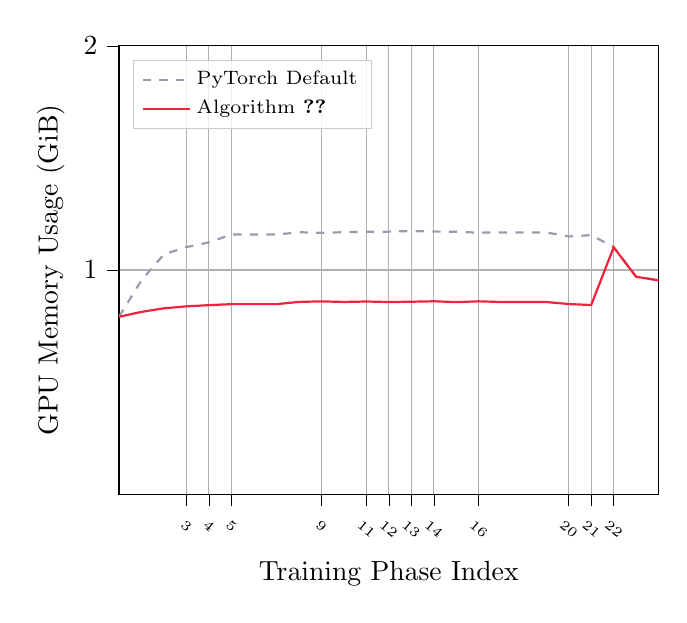
\begin{tikzpicture}

\definecolor{crimson2393560}{RGB}{239,35,60}
\definecolor{darkgray151157172}{RGB}{151,157,172}
\definecolor{darkgray176}{RGB}{176,176,176}
\definecolor{lightgray204}{RGB}{204,204,204}

\begin{axis}[
legend cell align={left},
legend style={fill opacity=0.8, draw opacity=1, text opacity=1, draw=lightgray204},
tick align=outside,
tick pos=left,
title={ },
x grid style={darkgray176},
xlabel={Training Phase Index},
xmajorgrids,
xmin=0, xmax=24,
xtick style={color=black},
xticklabel style={rotate=340.0},
ytick={1,2},
xtick={3,4,5,9,11,12,13,14,16,20,21,22},
xticklabel style={rotate=340.0, font=\tiny},
legend style={font=\scriptsize, at={(0,1)},anchor=north west, xshift=5pt,yshift=-5pt},
y grid style={darkgray176},
ylabel={GPU Memory Usage (GiB)},,
ymajorgrids,
ymin=0, ymax=2,
ytick style={color=black}
]
\addplot [thick, darkgray151157172, dashed]
table {%
0 0.79103125
1 0.95390625
2 1.06978125
3 1.10209375
4 1.12321875
5 1.15784375
6 1.15784375
7 1.15784375
8 1.16834375
9 1.16584375
10 1.16846875
11 1.17046875
12 1.17095703125
13 1.1738837890625
14 1.1712705078125
15 1.1704580078125
16 1.1664580078125
17 1.1673330078125
18 1.1673330078125
19 1.1673330078125
20 1.1493330078125
21 1.1553955078125
22 1.1019580078125
23 0.9702392578125
24 0.9543955078125
};
\addlegendentry{PyTorch Default}
\addplot [thick, crimson2393560]
table {%
0 0.79103125
1 0.81303125
2 0.828875
3 0.83778125
4 0.8430625
5 0.8475625
6 0.8475625
7 0.8475625
8 0.8574375
9 0.85990625
10 0.857328125
11 0.859328125
12 0.85701953125
13 0.8583056640625
14 0.8603173828125
15 0.8565517578125
16 0.8601767578125
17 0.8570517578125
18 0.8570517578125
19 0.8570517578125
20 0.8480517578125
21 0.8435517578125
22 1.1011767578125
23 0.9694580078125
24 0.9536142578125
};
\addlegendentry{Algorithm~\ref{alg:dynamic-checkpoint-selection}}
\end{axis}
\end{tikzpicture}


    \caption{GPU Memory Usage Profiling on Plain AlexNet with The Optimal Set of Checkpoints, \{3, 4, 5, 9, 11, 12\}.} 
    \label{fig:GMU_AlexNet_Ckpt_Optimal}
\end{figure}